\chapter{Further Plots}


\begin{Schunk}
\begin{Sinput}
>     library(norMmix, lib.loc="~/ethz/BA/norMmix.Rcheck/")
>     mainsav <- normalizePath("~/ethz/BA/Rscripts/")
\end{Sinput}
\end{Schunk}

\section{Behaviour in $n$}
\label{app:ben}

Here are the further plots ommited in section \ref{sec:ben}.
First is a very difficult mixture, ommited because it is studied in greater 
detail in section \ref{sec:def}. Second is a very easy mixture, because all
fitting lines overlap, making meaningful analysis futile.

\subsection{{\tt MW214}}

\begin{Schunk}
\begin{Sinput}
>     MW214
\end{Sinput}
\begin{Soutput}
norMmix object: 
multivariate normal mixture model with the following attributes:
name: 		 #14 Smooth Comb 
 model: 		 VII 
 dimension:	 2 
 components:	 6 
weight of components 0.5 0.1 0.1 0.1 0.1 0.1 
\end{Soutput}
\end{Schunk}


\begin{figure}[h!]
    \centering
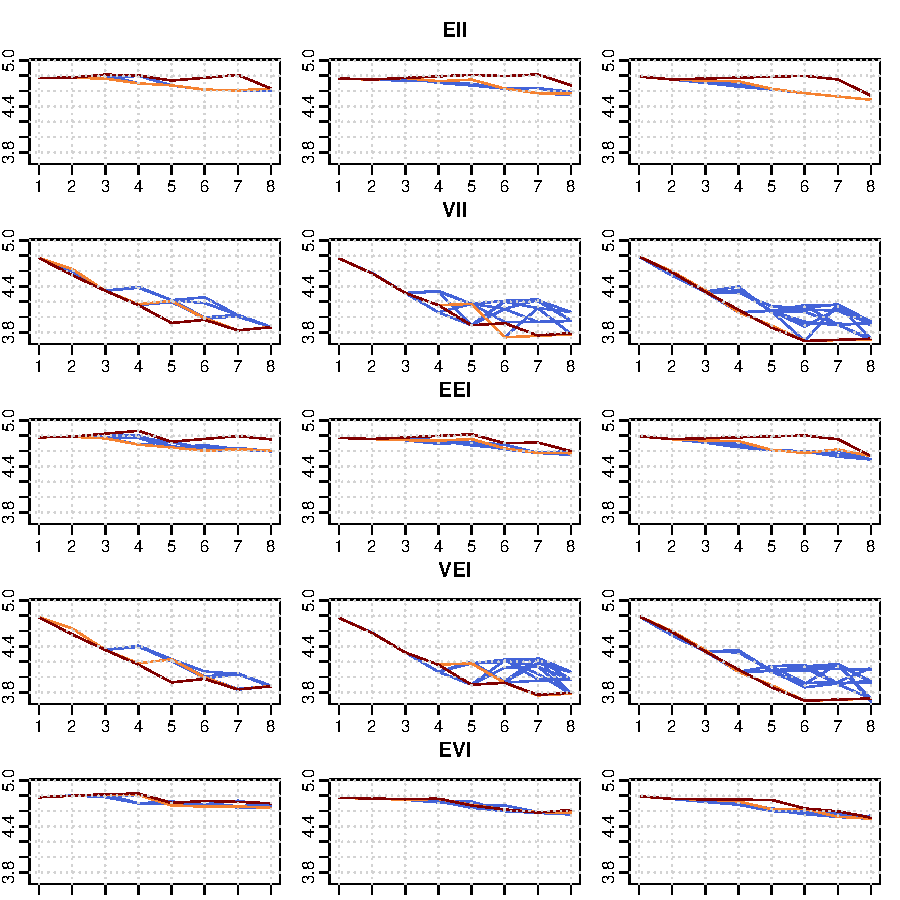
\includegraphics{App_plots-figmw21bicfirst}
    \caption{BIC values of {\tt MW214} with $n=\{500, 1000, 2000\}$, first five models}
    \label{fig:bicmw34first}
\end{figure}

\begin{figure}[h!]
    \centering
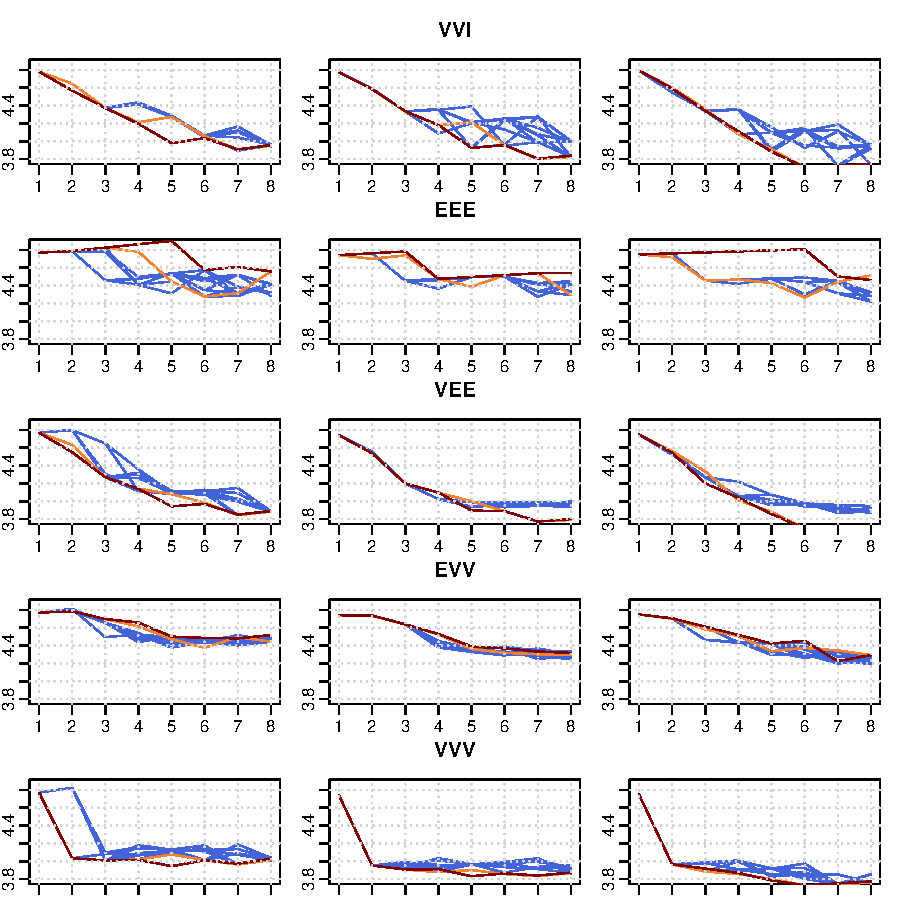
\includegraphics{App_plots-figmw21bicsecond}
    \caption{BIC values of {\tt MW214} with $n=\{500, 1000, 2000\}$, last five models.}
    \label{fig:bicmw34second}
\end{figure}

\clearpage

\subsection{{\tt MW51}}

\begin{figure}[h!]
    \centering
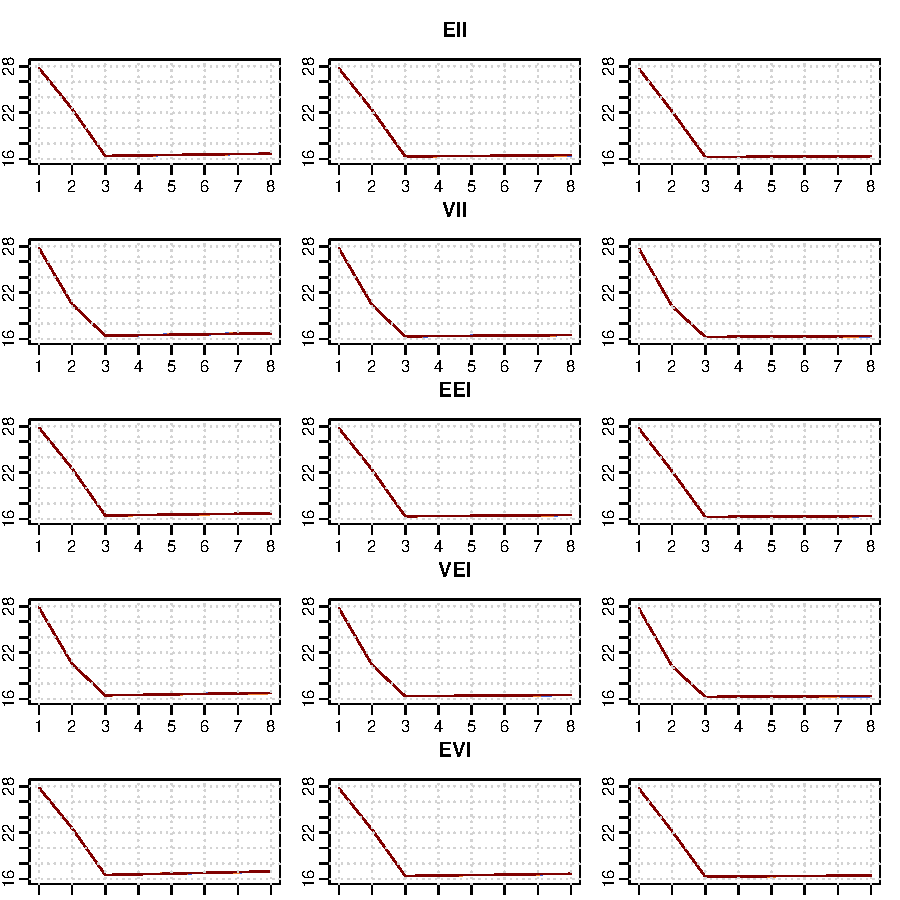
\includegraphics{App_plots-figmw51bicfirst}
    \caption{BIC values of {\tt MW51} with $n=\{500, 1000, 2000\}$}
    \label{fig:bicmw34first}
\end{figure}

\begin{figure}[h!]
    \centering
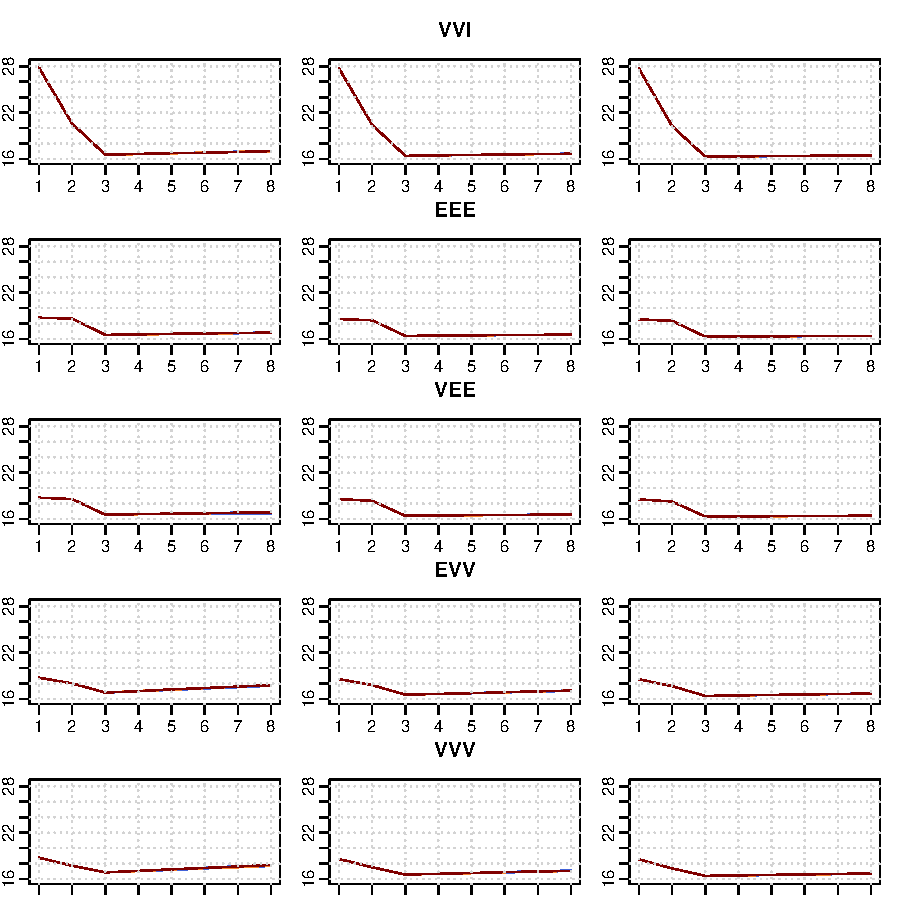
\includegraphics{App_plots-figmw51bicsecond}
    \caption{BIC values of {\tt MW51} with $n=\{500, 1000, 2000\}$}
    \label{fig:bicmw34second}
\end{figure}

\clearpage

\section{Other Data}

Unfortunately not all simulations were as useful to show in the main body of 
this work. In part, because they were done for exploratory purposes. However,
they show some other properties that are of interest.

The data in {\tt /simulations/smallinit} varied the dataset with a set seed.
The values for every individual dataset are not as interesting as 
{\tt /simulations/2time}, but they show that {\tt norMmix} is consistent in its
results for similar datasets.


\begin{figure}
    \centering
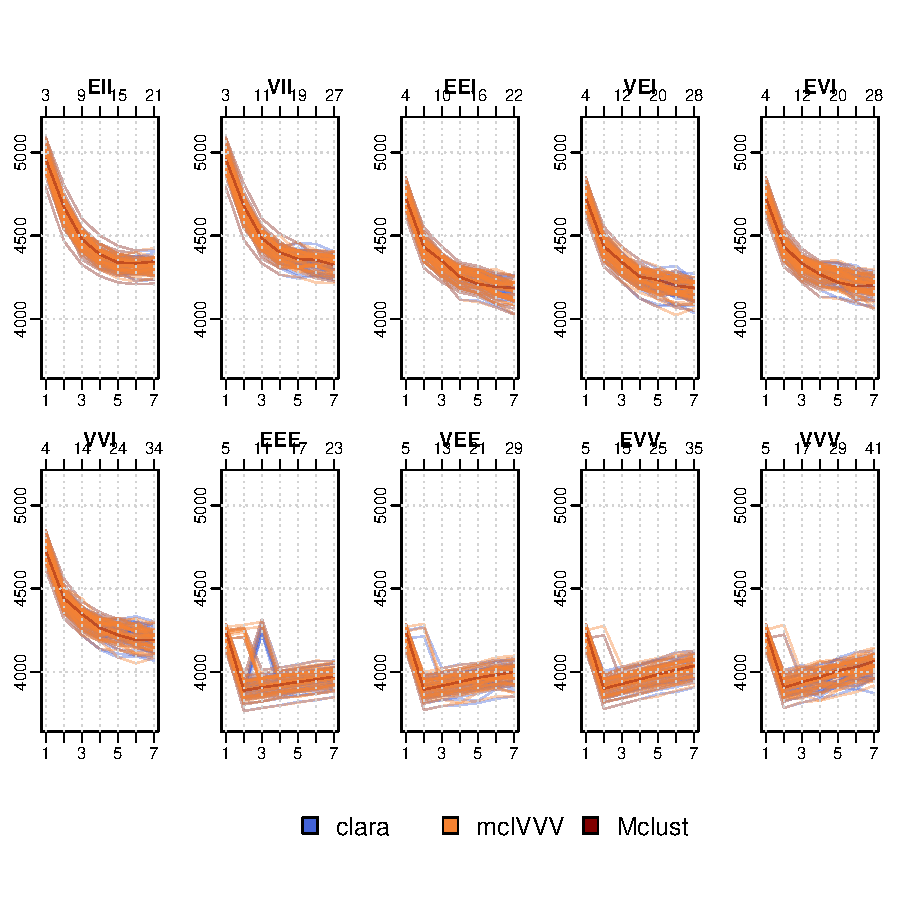
\includegraphics{App_plots-009}
\end{figure}

\begin{figure}
    \centering
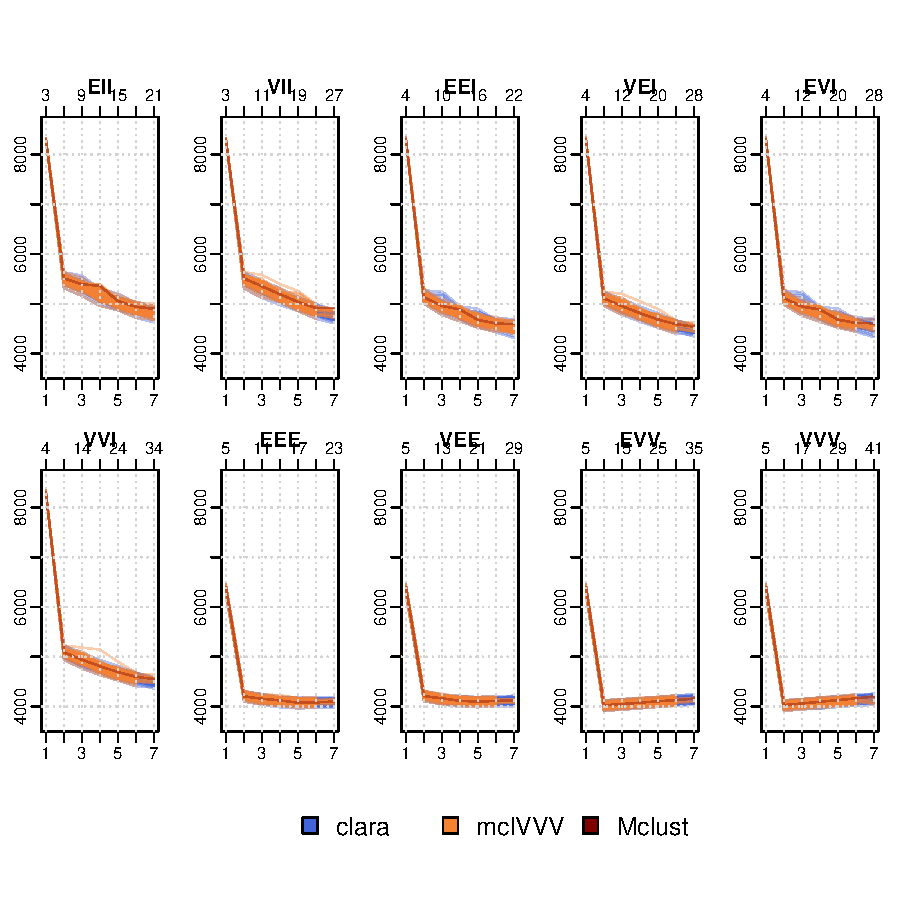
\includegraphics{App_plots-010}
\end{figure}

\begin{figure}
    \centering
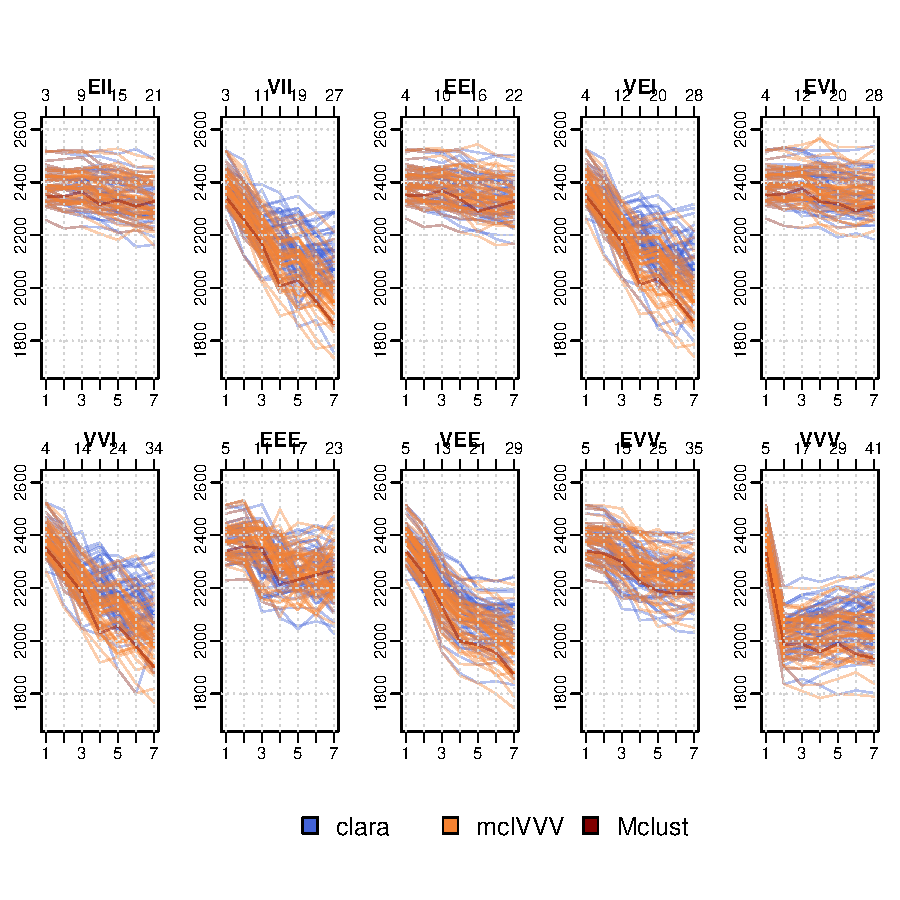
\includegraphics{App_plots-011}
\end{figure}

\begin{figure}
    \centering
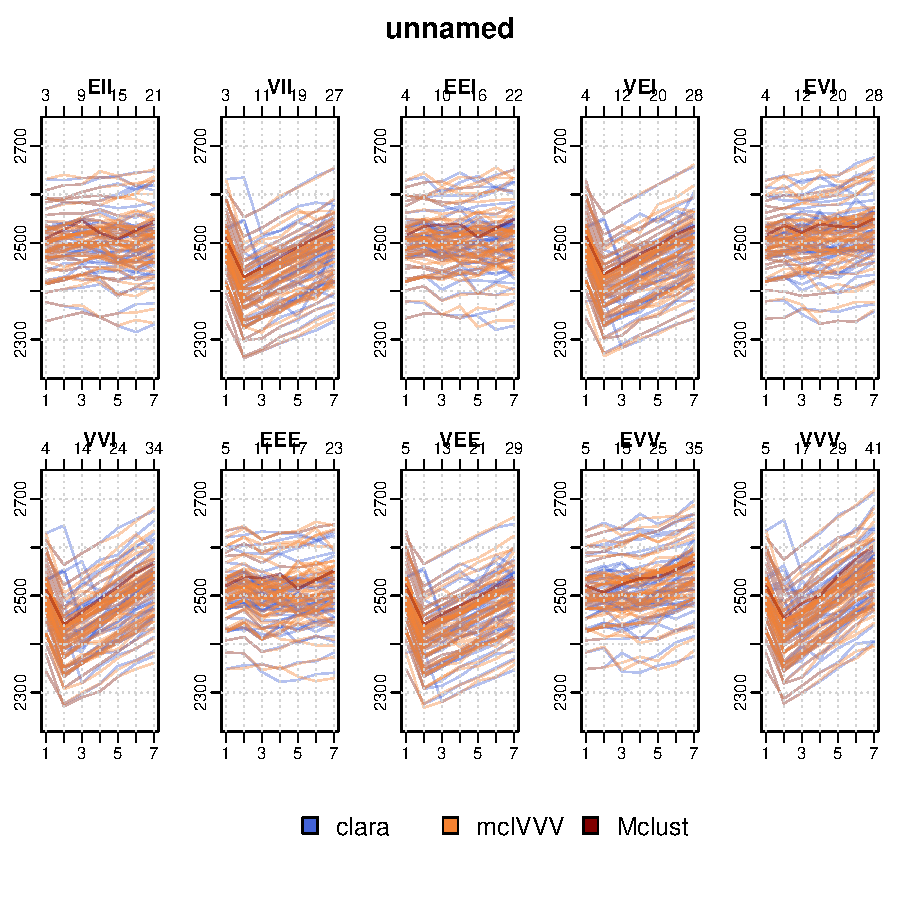
\includegraphics{App_plots-012}
\end{figure}

\begin{figure}
    \centering
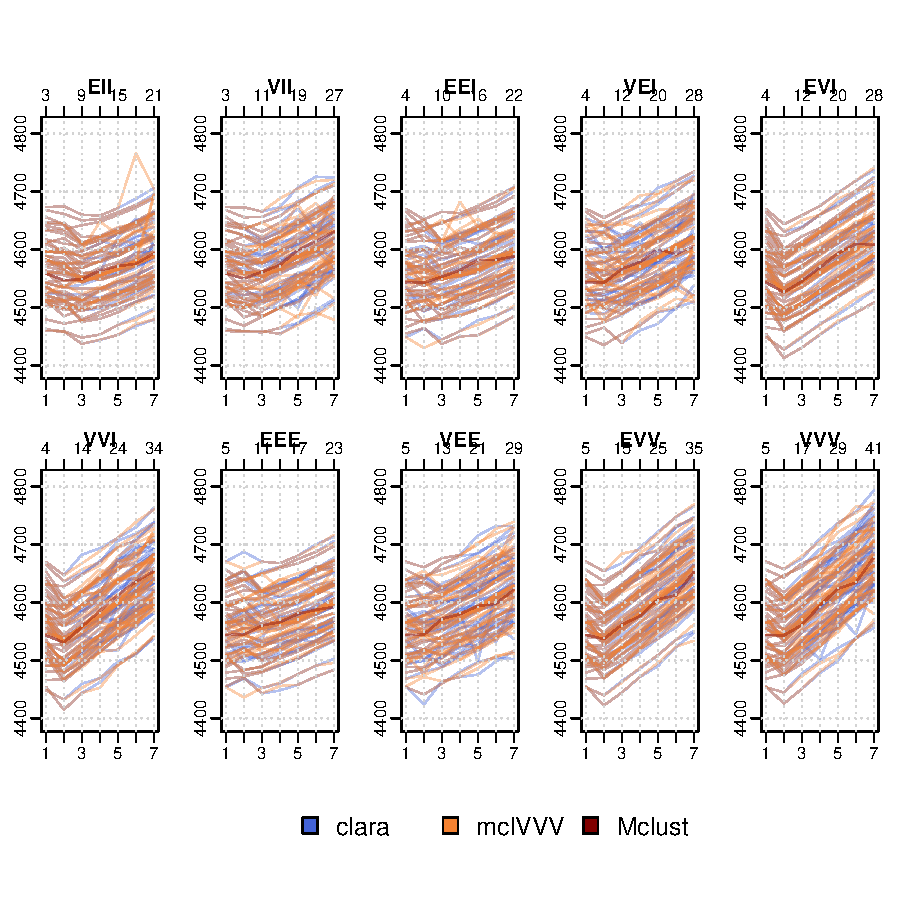
\includegraphics{App_plots-013}
\end{figure}

\begin{figure}
    \centering
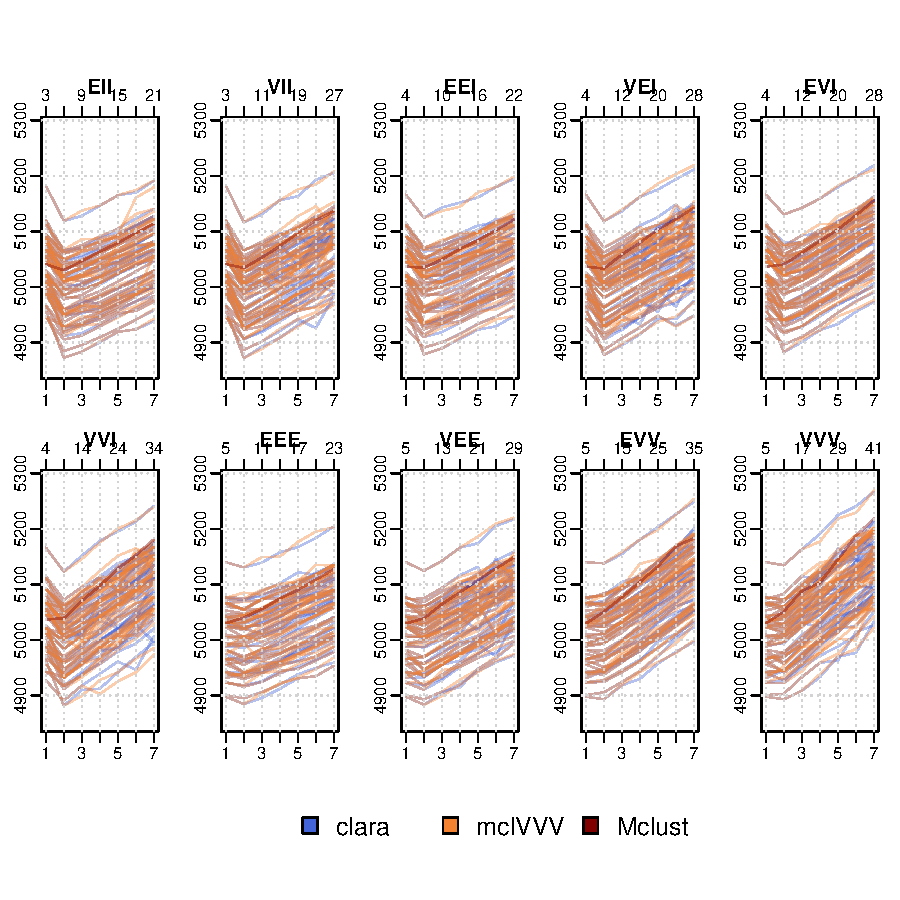
\includegraphics{App_plots-014}
\end{figure}
